\documentclass{beamer}

\usetheme{default}
\usecolortheme{rose}
\usepackage{hyperref}
\newcommand{\ignore}[1]{}
\newcommand{\pr}{\mathbb{P}}
\newcommand{\E}{\mathbb{E}}
\newcommand{\sd}{\text{sd}}
\newcommand{\var}{\text{var}}
\setbeamerfont{alerted text}{series=\itshape}
\addtobeamertemplate{navigation symbols}{}{%
    \usebeamerfont{footline}%
    \usebeamercolor[fg]{footline}%
    \hspace{1em}%
    \insertframenumber/\inserttotalframenumber
}

\title{The Central Limit Theorem and Confidence Intervals}

% A subtitle is optional and this may be deleted
\subtitle{STAT-UB.0001 Statistics for Business Control}

\author{Ningshan Zhang}
% - Give the names in the same order as the appear in the paper.
% - Use the \inst{?} command only if the authors have different
%   affiliation.

\institute[New York University] % (optional, but mostly needed)
{
  IOMS Department\\
  nzhang@stern.nyu.edu
  \let\thefootnote\relax\footnotetext{\tiny{*  Office Hours: Wed \& Fri 10:00 - 11:30 AM, KMC 8-174}}
}
\date{Jul 26, 2018}
\AtBeginSubsection[]
{
  \begin{frame}<beamer>{Outline}
    \tableofcontents[currentsection,currentsubsection]
  \end{frame}
}

% Let's get started
\begin{document}

%-------------------
\begin{frame}
  \titlepage
\end{frame}



% Section and subsections will appear in the presentation overview
% and table of contents.
%-------------------
\begin{frame}{Review}
Continuous random variables
\begin{itemize}
\item Probability density function (pdf)
\item Area under the curve
\end{itemize}
\vspace{\stretch{0.2}}
Normal distribution
\begin{itemize}
\item Normal distribution's pdf
\item Standard normal distribution, z-tables
\item Convert normal to standard normal
\end{itemize}
\end{frame}

%\begin{frame}{Sampling}
%\end{frame}

%-------------------
\begin{frame}{Populations and Samples}
There are many times that we want to know something about a population, but it is unrealistic to gather all the information to obtain an exact answer.

\vspace{\stretch{0.2}}
Example:
\begin{itemize}
\item What is the average amount of time that NYU undergraduates spend text messaging per day?
\item What is the average income of all Stern graduates?
\end{itemize}
\end{frame}

%-------------------
\begin{frame}{Populations and Samples}
As an alternative, we can take a random subset of items or individuals from the population, 
and use this random sample to draw conclusions about the population.

\vspace{\stretch{0.2}}
\begin{itemize}
\item A random subset is an unbiased sample of the population.
\item Will we get a precise answer to our original question?
\end{itemize}
\end{frame}

%-------------------
\begin{frame}{Population Parameters and Sample Statistics}
Population parameters
\begin{itemize}
\item Descriptive measures of a \alert{population}
\item Example: population mean, population variance
\end{itemize}

\vspace{\stretch{0.2}}
Sample statistics
\begin{itemize}
\item Descriptive measures of a \alert{sample}
\item Example: sample mean, sample variance
\end{itemize}

\vspace{\stretch{0.2}}
Goal: use sample statistics to make inferences about the parameters of a population.
\end{frame}

%-------------------
\begin{frame}{Population Parameters and Sample Statistics}
Often, sample statistics are estimators of population parameters.
\begin{table}\begin{center}
\begin{tabular}{ |c|c|}
\hline
Population parameter  & Sample statistic \\\hline
$\mu$ & $\bar x$ \\ \hline
$\sigma^2$ & $s^2$\\ \hline
$\sigma$ &  $s$ \\ \hline
$p$ & $\hat p$ \\ \hline
\end{tabular}
\end{center}\end{table}

\vspace{\stretch{0.4}}
However, sample statistics are subject to randomness.
\begin{itemize}
\item Different samples will give different estimates.
\item Estimates are (almost) never exactly correct.
\end{itemize}
\let\thefootnote\relax\footnotetext{\tiny{* 
\href{https://www.stat.auckland.ac.nz/~wild/WPRH/AnimGifs/CompareSampSize.gif}{Link to Animations of Sampling Variation}}}

\end{frame}

%-------------------
\begin{frame}{Sampling Distribution}
Sample statistic is a random variable:
\begin{itemize}
\item Random experiment: randomly draw $n$ observations from the population.
\item Outcome of the random experiment: sample statistic calculated from the sample of $n$ observations.
\end{itemize}

\vspace{\stretch{0.4}}
Since sample statistic is a random variable it follows some distribution.  
We refer to this distribution as a \alert{sampling distribution}.
\end{frame}

%-------------------
\begin{frame}{Populations and Samples}
\begin{center}
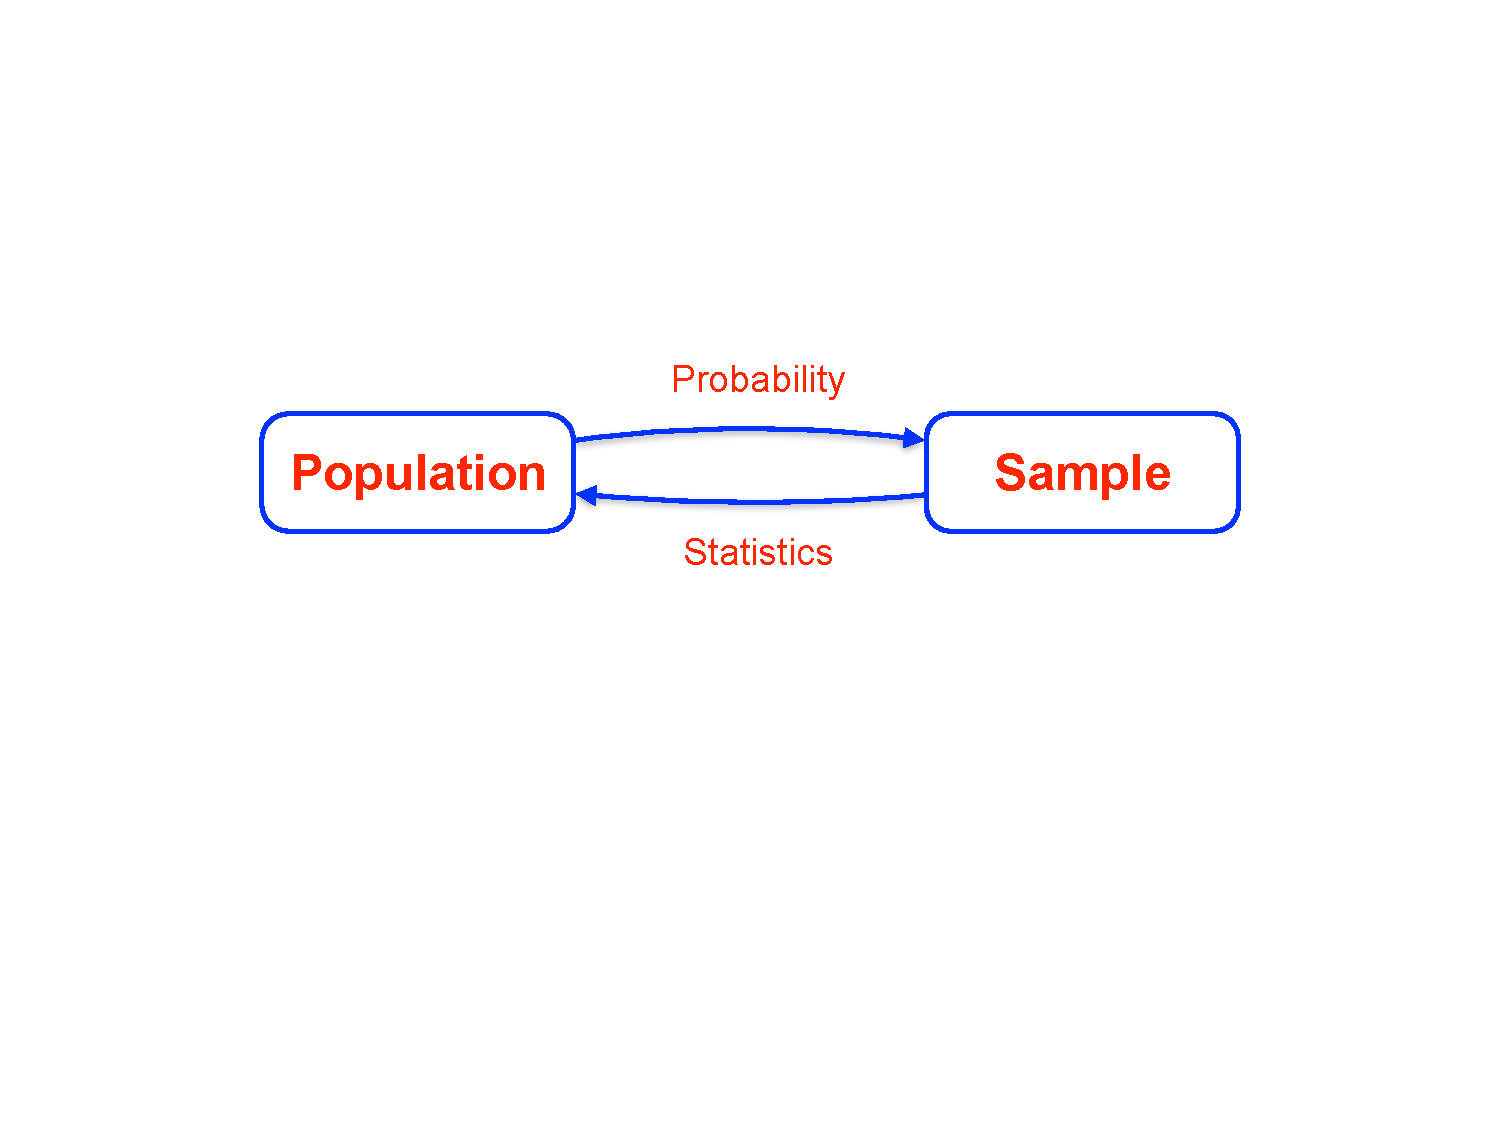
\includegraphics[width=0.8\textwidth]{figures/prob_and_stat.pdf}
\end{center}
\begin{itemize}
\item Probability: how would the sample statistic fluctuate around the population parameter?
\item Statistics: given the sample, what are possible values of the population parameter?
\end{itemize}
\end{frame}


%-------------------
\begin{frame}{Sampling Distribution of Sample Mean $\bar X$}
    Given a sample of $n$ observations, $X_1,\cdots, X_n$, the sample mean is computed as
    $$\bar X = \frac{1}{n} \sum_{i=1}^n X_i.$$

\vspace{\stretch{0.2}}
We will study the sampling distribution of $\bar X$:
\begin{itemize}
    \item Expected value of $\bar X$, denoted by $\E (\bar X)$ or $\mu_{\bar x}$.
    \item Standard deviation of $\bar X$, denoted by $\sd (\bar X)$ or $\sigma_{\bar X}$.
    \item Histogram of $\bar X$.
\end{itemize}
\end{frame}

%-------------------
\begin{frame}{The Central Limit Theorem (CLT)}
    Suppose $X_1,X_2,\dots,X_n$ are sampled independently from a population with mean $\mu$ and 
    standard deviation $\sigma$. Let $\bar X$ be the sample mean, 
    $$\bar X = \frac{1}{n} \sum_{i=1}^n X_i.$$
    Then,
    \begin{itemize}
        \item  $\mu_{\bar X}= \E(\bar X) = \mu$,
        \item $\sigma_{\bar X} =\sd(\bar X) =  \frac{\sigma}{\sqrt{n}}$,
        \item  If $n$ is sufficiently large ($n\geq 30$), then $\bar X$ is approximately normal.
    \end{itemize}
\end{frame}

%-------------------
\begin{frame}{Expected Value of $\bar X$}
    The expected value of $\bar X$ is $\mu$:
    \begin{align*}
        \mu_{\bar X} & = \E\Big( \frac{1}{n} \sum_{i=1}^n X_i\Big) 
                     = \frac{1}{n} \sum_{i=1}^n \E(X_i) 
                     = \mu.
    \end{align*}

\vspace{\stretch{0.2}}
\begin{itemize}
    \item We will refer to $\mu_{\bar X}$ as the ``mean of sample mean''.
%    \item Since the expected value of $\bar X$ is the true population mean $\mu$, $\bar X$ is said to be an \alert{unbiased} estimator.
\end{itemize}
\end{frame}

%-------------------
\begin{frame}{Standard Deviation of $\bar X$}
    The standard deviation of $\bar X$ is $\sigma_{\bar X} = \frac{\sigma}{\sqrt{n}}$.

\vspace{\stretch{0.2}}
\begin{itemize}
    \item We will refer to $\sigma_{\bar X}$ as the ``standard deviation of sample mean''.
    \item The variance of $\bar X$ is $\frac{\sigma^2}{n}$.
\end{itemize}
\end{frame}


%-------------------
\begin{frame}{Distribution of $\bar X$}
    When $n$ is sufficiently large, $\bar X$ is approximately normally distributed, 
    with mean $\mu_{\bar X} = \mu$ and standard deviation $\sigma_{\bar X} = \frac{\sigma}{\sqrt{n}}$.

    \begin{itemize}
        \item In general, $n \geq 30$ is sufficiently large.
        \item $\bar X$ is approximately normal, even if the population is not.
        \item   $\bar X$ fluctuates around population mean $\mu$:
        $$ \pr(\mu-\frac{2\sigma}{\sqrt{n}} < \bar X < \mu+\frac{2\sigma}{\sqrt{n}}) = 0.95.$$

    \end{itemize}
    
\end{frame}


%-------------------
\begin{frame}{Distribution of $\bar X$}
    What if $n<30$?
    \begin{itemize}
        \item We need additional assumptions about the population distribution, in order to understand the distribution of $\bar X$.
    \end{itemize}

    \begin{table}\caption{Relationship between population and sample mean.}
        \begin{center}
            \begin{tabular}{|c|c|c|}
                \hline
                \textbf{Population} & \textbf{Sample size $n$} & \textbf{Sample mean $\bar X$} \\\hline
                Normal & any $n\geq 1$ & Normal \\\hline
                Any distribution & $n\geq 30$ & Approximately normal \\\hline
            \end{tabular}
        \end{center}\end{table}

\end{frame}


%-------------------
\begin{frame}{CLT Demo}
    This website has a nice demo of the Central Limit Theorem:
    \url{http://onlinestatbook.com/stat_sim/sampling_dist}

\vspace{\stretch{0.4}}
Try the following settings:
\begin{itemize}
    \item Set the population to be skewed, set $n=25$.
    \item Set a custom population, set $n=25$.
    \item Set a custom population, set $n=5$.
    \item Set the population to be normal, set $n=5$.
\end{itemize}
\end{frame}

%-------------------
\begin{frame}{Estimation}
    In practice we rarely know the true value of the population parameters, but we can use sample data to estimate them.
    \vspace{\stretch{0.2}}
    \begin{itemize}
            \item Point estimation: use a single number to estimate the population parameter of interest.
            \item Interval estimation: construct an interval that contains the true parameter value with a certain probability.
    \end{itemize}
\end{frame}

%-------------------
\begin{frame}{Point Estimation}
    Example:
    \begin{itemize}
        \item  $\bar X$ is a point estimator of $\mu$.
        \item $s^2$ is a point estimator of $\sigma^2$.
    \end{itemize}

    \vspace{\stretch{0.2}}
    Point estimates are problematic:
    \begin{itemize}
        \item (Almost) never exactly correct.
        \item Tell us nothing about their own variability.
    \end{itemize}
\end{frame}

%-------------------
\begin{frame}{Interval Estimation}
    Confidence Intervals:

    \vspace{\stretch{0.1}}
    \begin{itemize}
    \item A \alert{confidence interval} (CI) is a formula that tells us how to construct an interval using sample data, 
        such that the interval contains the true parameter value with a certain probability.
    \vspace{\stretch{0.1}}
    \item The formula varies depending on the the sample size, and the information available about the population.
    \end{itemize}
\end{frame}

%-------------------
\begin{frame}{Interval Estimation}
    We will study the following cases:
    \begin{itemize}
    \vspace{\stretch{0.1}}
    \item Confidence intervals for population mean $\mu$
    \begin{itemize}
    \vspace{\stretch{0.1}}
            \item Known population variance vs.\ unknown population variance
    \vspace{\stretch{0.2}}
            \item Large sample vs.\ small sample
    \end{itemize}
    \vspace{\stretch{0.1}}
    \item Confidence intervals for population proportion $p$
    \end{itemize}
\end{frame}

%-------------------
\begin{frame}{CI for the Mean: Known Variance}
    Setup: assume the population variance $\sigma^2$ is known, build a CI for the population mean $\mu$ using a sample of $n$ observations.

    \vspace{\stretch{0.1}}
    \begin{itemize}
        \item By CLT, when $n\geq30$, $\bar X$ is (roughly) normally distributed with mean $\mu$ and standard deviation $\sigma/\sqrt{n}$.
        \item Let $Z=\frac{\bar X - \mu}{\sigma/\sqrt{n}}$, then $Z$ is a standard normal (roughly).
    \item In particular,
        $$ \pr(-1.96 < \frac{\bar X - \mu}{\sigma/\sqrt{n}} < 1.96) = 0.95.$$
    \end{itemize}
\end{frame}


%-------------------
\begin{frame}{CI for the Mean: Known Variance}
    Rewrite the expression:
    \begin{align*}
        & \pr(-1.96 < \frac{\bar X - \mu}{\sigma/\sqrt{n}} < 1.96) = 0.95 \\
        \iff \ & \pr (\bar X - \frac{1.96 \sigma}{\sqrt{n}} < \mu < 
        \bar X + \frac{1.96 \sigma}{\sqrt{n}}) = 0.95
    \end{align*}

    \vspace{\stretch{0.1}}
    Thus, the interval $(\bar X - \frac{1.96 \sigma}{\sqrt{n}},\bar X + \frac{1.96 \sigma}{\sqrt{n}})$ is 
    a CI for $\mu$ with confidence level $0.95$.
\end{frame}

\begin{frame}{CI for the Mean: Known Variance}
    In general, let $z_{\alpha/2}$ be the value such that 
    $$ \pr(-z_{\alpha/2} < Z < z_{\alpha/2})=1-\alpha. $$
\begin{columns}[T] % align columns
\begin{column}{.4\textwidth}
    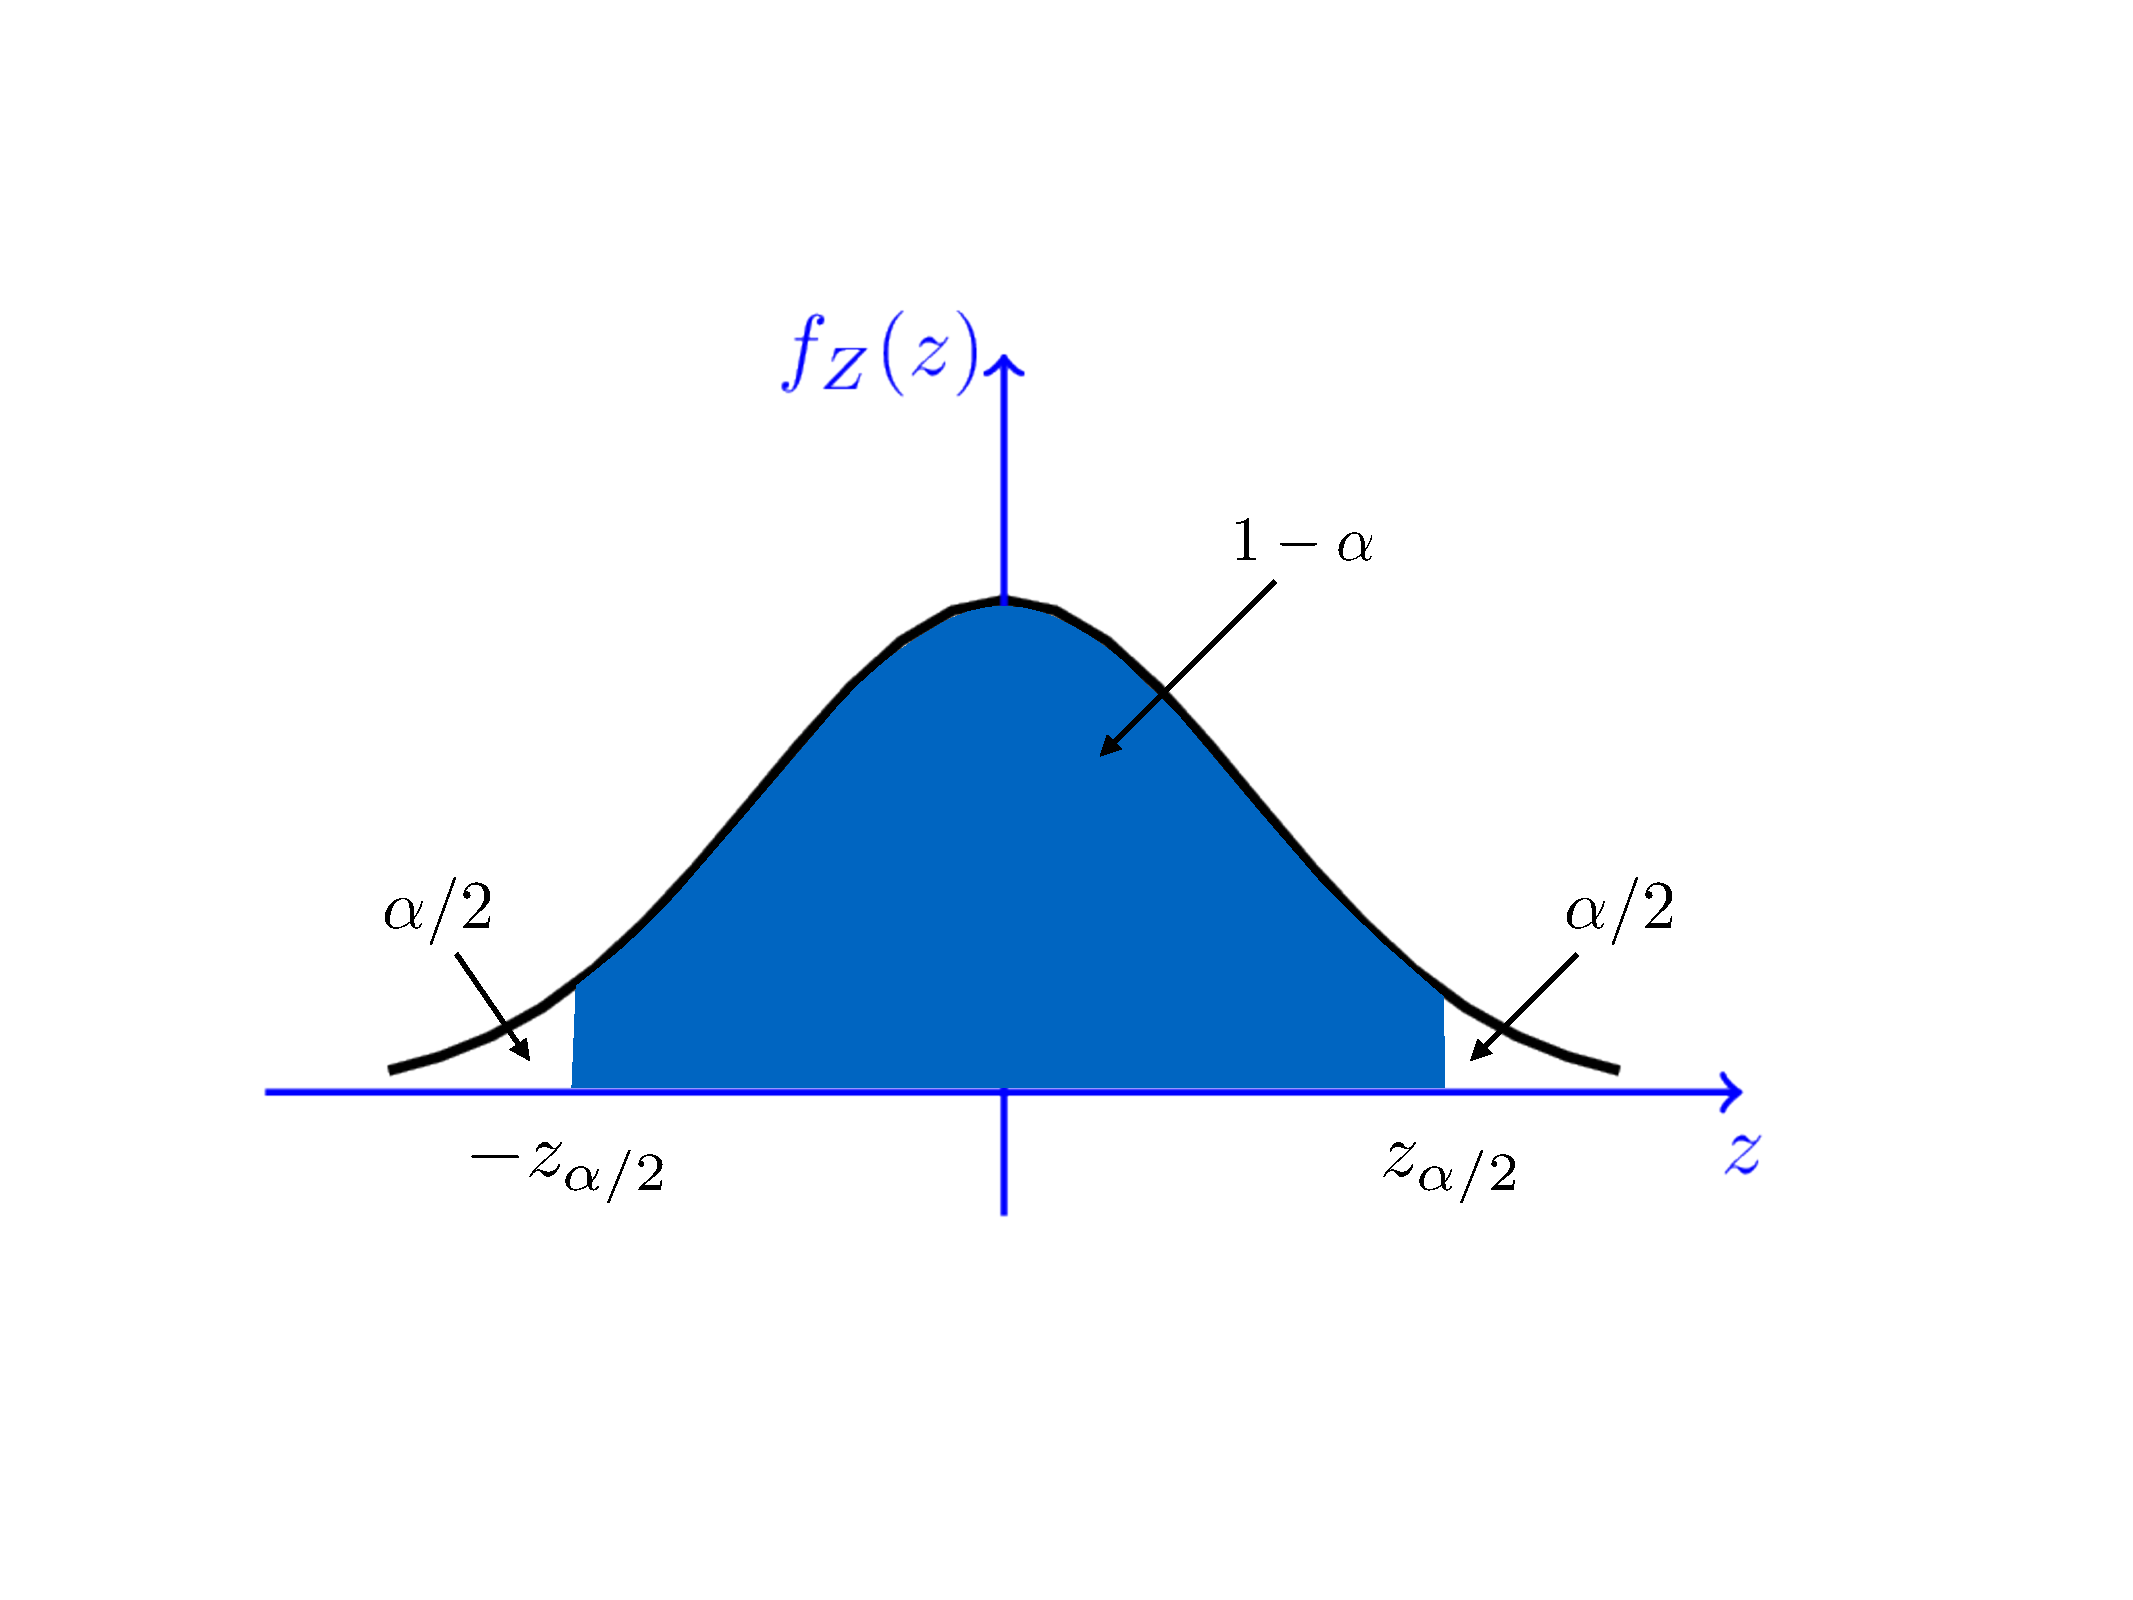
\includegraphics[width=1\textwidth]{figures/zscore}
\end{column}%
\hfill%
\begin{column}{.5\textwidth}
\vspace{0.15in}
Example:
\begin{itemize}
\item $\alpha=0.05$, $z_{0.025} = 1.96.$ 
\item $ \alpha=0.1$, $z_{0.05} =  1.64.$
\end{itemize}
\end{column}%
\end{columns}

\vspace{0.05in}
    Then the interval $(\bar X - z_{\alpha/2}\dfrac{\sigma}{\sqrt{n}},\bar X + z_{\alpha/2}\dfrac{\sigma}{\sqrt{n}})$ is a CI for $\mu$ with confidence level $1 –\alpha$.
\end{frame}

%-------------------
\begin{frame}{Example}
In an attempt to estimate the average number of sick days an employee uses in a year in a large firm, 
a HR manager examined a sample of 200 employees. Sample average was $\bar X= 3.47$.  
Assuming a population standard deviation of $\sigma= 2.8$ days, build a 90\% CI for $\mu$, the true average among all employees.
\end{frame}

%-------------------
\begin{frame}{Interpretations of Confidence Intervals}
In the example, we found that $(3.14, 3.80)$ is a 90\% CI for $\mu$. 

\vspace{\stretch{0.2}}
Which of the following statements is true?
\begin{enumerate}[(a)]
\item There is a 0.90 probability that $\mu$ is between 3.14 and 3.80.
\item $\mu$ will be between 3.14 and 3.80 90\% of the time.
\item In 90\% of all future samples, $\bar X$ will be between 3.14 and 3.80.
\item  $\mu$ is between 3.14 and 3.80.
\item None of the above.
\end{enumerate}
\end{frame}

%-------------------
\begin{frame}{Interpretations of Confidence Intervals}
\alert{Warning: The practical interpretation of a CI is tricky!}

\vspace{\stretch{0.2}}
\begin{itemize}
\item $\mu$ is nonrandom, it makes no sense to talk about the probability of $\mu$.
\item The ``$1-\alpha$ confidence level'' refers to the process of constructing confidence intervals, not to the particular CI estimate obtained from the given sample.
\end{itemize}
\end{frame}

%-------------------
\begin{frame}{Interpretations of Confidence Intervals}
The proportion of these intervals (in the long run) that contain $\mu$ is equal to $1-\alpha$.
\begin{figure}\caption{Different samples give different CIs.}
    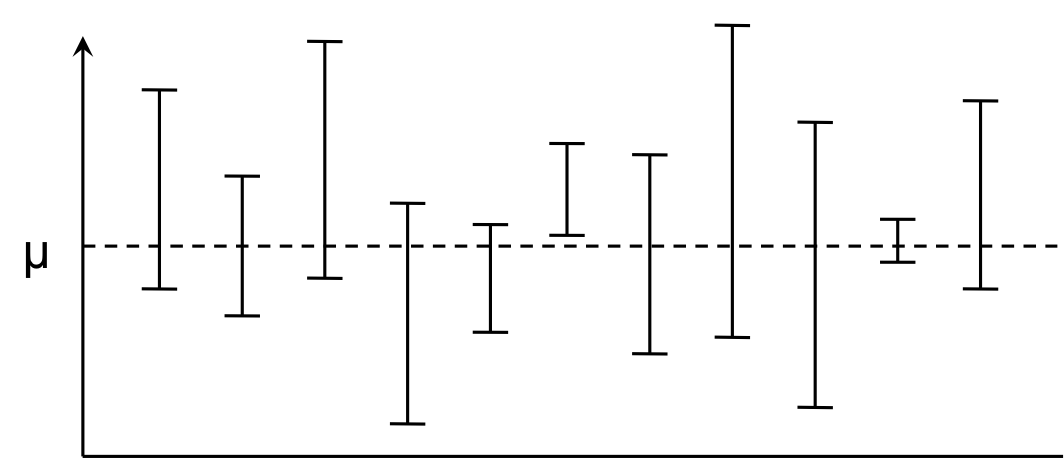
\includegraphics[width=0.8\textwidth]{figures/CI.png}
\end{figure}
\end{frame}

%-------------------
\begin{frame}{Interpretations of Confidence Intervals}
In practice, we only have one sample, so why should we care about confidence intervals?
\begin{itemize}
\item $1-\alpha$ represents the proportion of times that we successfully obtain a CI that covers $\mu$.
\item Generally, we make $\alpha$ small so that most of the confidence intervals that we compute will contain $\mu$.
\end{itemize}

\vspace{\stretch{0.2}}
Why not construct a 100\% confidence interval?
\end{frame}

%-------------------
\begin{frame}{Interpretations of Confidence Intervals}
Compare: the price a customer will be willing to pay for our new, revolutionary cell phone is between
\begin{itemize}
\item \$0 and \$250 M, with 100\% certainty.
\item \$355 and \$420 M, with 90\% certainty.
\end{itemize}

\vspace{\stretch{0.2}}
The price of higher certainty is lack of accuracy.
\end{frame}



%-------------------
%\begin{frame}{CI for the Mean: \alert{Unknown} Variance}
%\begin{itemize}
%\item So far, when $\sigma$ is known the interval  
%$$ (\bar X - z_{\alpha/2}\dfrac{\sigma}{\sqrt{n}},\bar X + z_{\alpha/2}\dfrac{\sigma}{\sqrt{n}})$$
%    is a CI for $\mu$, with confidence level $1-\alpha$.
%\item    Unfortunately, the assumption that $\sigma$ is known is unrealistic in many situations. 
%\item   In practice, we typically use $s$, the \alert{sample standard deviation}, to estimate $\sigma$.
%\end{itemize}
%\end{frame}

%-------------------
\ignore{
\begin{frame}{Time Series Plot}
\begin{figure}
    \caption{}
    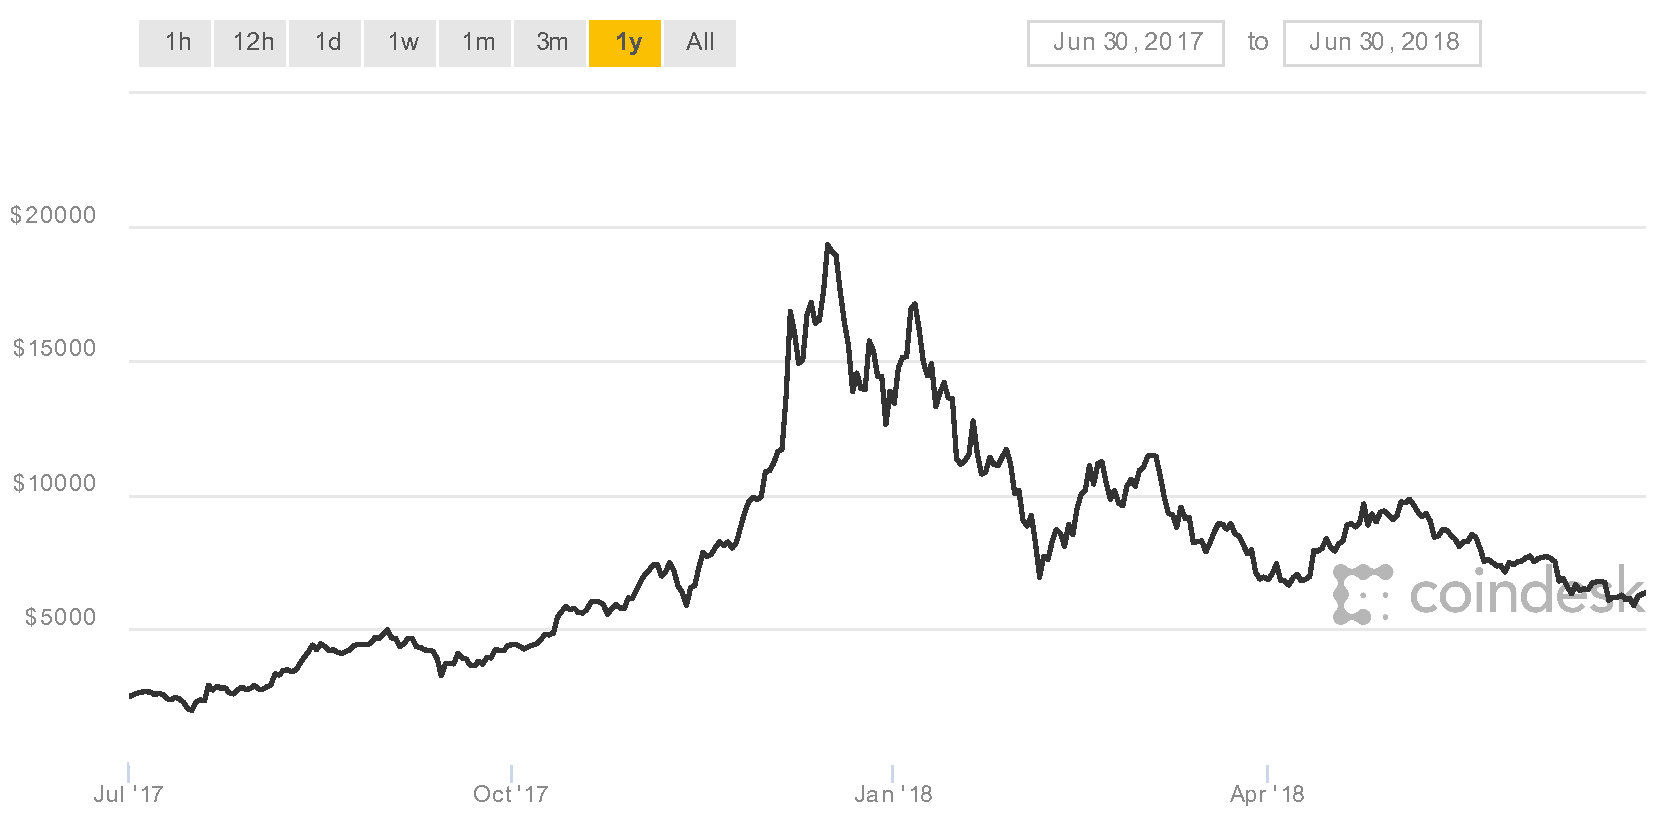
\includegraphics[width=1\textwidth]{figures/coindesk-bpi-chart}
\end{figure}
\let\thefootnote\relax\footnotetext{\tiny{* Plot from Coindesk.com}}
\end{frame}

\begin{frame}{}
\begin{itemize}
\item 
\end{itemize}
\end{frame}

\vspace{\stretch{0.5}}

\begin{block}{}
\end{block}


}

\end{document}


